\chapter{Constructions}\label{chap:constructions}

\begin{epigraph}{14em}{Hermann Weyl}
	The introduction of numbers as \\
	coordinates is an act of violence.
\end{epigraph}

The focus on this chapter will be on three important constructions of exotic spheres -- as total spaces of sphere bundles, as the boundary of a ``plumbing'' of disk bundles along a tree, and as the ``link'' of an isolated singularity of a holomorphic functions. In later sections, it will be possible to directly compute invariants of these constructed manifolds to understand which elements of $\Theta^n$ these manifolds correspond to. As with many challenging topics in math, an abundance of examples helps alleviate some of the complexity, and we hope this chapter can do this for exotic spheres.
That being said, a time-pressed reader need only read \cref{sec:plumbing}, since this is a simple direct construction which will suffice for a classification of exotic spheres in \cref{chap:classification}.

The basic ingredients for a good exotic sphere construction includes the following:
\begin{enumerate}[(a)]
	\item A general class of non-trivial smooth manifolds which have highly-connected boundary.
	\item A simple criterion for when this boundary is homotopy equivalent to a sphere.
	\item Some geometric structure on the bounding manifold which simplifies the computation of some topological invariants.
\end{enumerate}

\todo{connect}

If we require homotopy spheres to have a framed coboundary (i.e. restrict to $\bP^{n+1}\subset \Theta^n$), it turns out that the homotopy sphere is entirely determined by the intersection form of its coboundary. We will prove this in \cref{chap:classification}. For now, we note that since Pontryagin classes of a trivial bundle vanish, the invariants of \cref{sec:invariants-for-homotopy-4k-1-spheres} take the form
\[
	\lambda(M) = A\sigma(W)\mod B
\]
for some integers $A$ and $B$. Since the signature is additive with respect to connected sums, any time we construct a homotopy sphere $M$ with coboundary of signature $\sigma(W)$, we get a (non-exact) sequence of homomorphisms
\[
	\Z \lkxto \bP^{n+1} \lkxto[\lambda] \Z/B
\]
sending $t\in \Z$ to the iterated connected sum $\+[t] M\in \bP^{n+1}$. Since $ $

\pagebreak
\section{Milnor Spheres}\label{sec:milnor-spheres}

We will begin with the classical construction of exotic spheres as total spaces of bundles over a sphere, starting with Milnor's original construction of an exotic 7-sphere in \cite{milnor1956manifolds}.
To see how spheres can arise as total spaces of bundles over a sphere, we will review the Hopf bundles -- these construct ordinary spheres of dimensions $1$, $3$, $7$ (and $15$). By ``twisting'' Hopf bundles in sufficiently high dimension, we will be able to get exotic spheres, although such a construction only works in these dimensions. We will see in the following section how to generalize the construction by means of ``plumbing'' a string of bundles to get exotic spheres in arbitrary dimensions.

The simplest Hopf bundle is the real Hopf bundle, which constructs the circle $S^1$ as the total space of an $S^0$ bundle over $S^1$. Topologically, this is just the double cover of $S^1$, but it is instructive to consider this simple case in the same manner as the complex and quaternionic Hopf bundles which be considered next.
Consider the projection map
\[
	\lkxfunc{\pi_\R^n}{S^n}{\RP^n}{(x_1,\ldots, x_{n+1})}{[x_1:\cdots: x_{n+1}]}
\]
sending a point $p$ on a sphere $S^n\subset \R^{n+1}$ to the line passing through $p$ and the origin. This is a double cover since antipodal points on a sphere lie on the same line -- and in fact $S^n$ is the universal covering space of $\RP^n$ when $n>1$. The fibers of this map are thus the zero-dimensional sphere $S^0$. It is useful to interpret these fibers as the Lie group $\O_1\cong \Z/2$ consisting of linear transformations of a

When $n=1$, there is an isomorphism $\RP^1\approx S^1$ by stereographic projection, and so $\pi_\R^1$ is the $S^0$-bundle
\[
	S^0 \lkxto S^1\lkxto S^1.
\]
This is the \defn{real Hopf bundle}[Hopf bundle (real)].
Note that real Hopf bundle $\pi_\R^1$ can be interpreted as the boundary of the compact M\"obius bundle $M$, which is a $D^1$-bundle over $S^1$.

Advancing from $\R$ to $\C$, we next consider the projection map
\[
	\lkxfunc{\pi_\C^n}{S^{2n+1}}{\CP^n}{(z_1,\ldots, z_{n+1})}{[z_1:\cdots: z_n]}
\]
where we interpret $S^{2n+1}\subset \R^{2n+2}$ as a subset of $\C^{n+1}$. Rather than send a point to a real line, the map $\pi_\C^n$ sends a point $p\in \C^{n+1}$ on the complex unit sphere to the complex plane passing through the origin and $p$. Note that changing the ``phase'' of the point $p$ along the plane keeps the point in the plane. The fibers thus consist of phase changes, i.e. the Lie group $\U_1=\{e^{i\theta} : \theta\in \R\}$ which is diffeomorphic to $S^1$.

When $n=1$, there is an isomorphism of the Riemann sphere $\CP^1\cong S^2$ by stereographic projection. This gives the us the infamous \defn{complex Hopf bundle} $\pi_\C^1$
\[
	S^1 \lkxto S^3 \lkxto S^2.
\]

\begin{remark}
	Unlike the real and complex numbers, the ring of quaternions $\HH$ is not a field since it is not commutative. We define the quaternionic projective space $\HP^{n}$ as the quotient of $\HH^{n+1}$ by \emph{right} multiplication by $\HH$.
\end{remark}

In the final case of the quaternionic plane $\HH$, we have a projection map
\[
	\lkxfunc{\pi_\HH^n}{S^{4n+3}}{\HP^n}
\]
where we consider $S^{4n+3}\subset \HH^{n+1}$. This bundle with fibers given by the set of unit quaternions $S^3\subset \HH$.
In the case $n=1$, the difeomorphism $\HP^1\cong S^3$ gives the \defn{quaternionic Hopf bundle}[Hopf bundle (quaternionic)]
\[
	S^3 \lkxto S^7 \lkxto S^4.
\]
As before, the fiber $S^3$ should be interpreted as the Lie group $\Sp_1$ of unit quaternions. These act as quaternionic phase shifts.

Now let $\F\in\{\R, \C, \HH\}$, and $d=\dim_\R \F$ be the dimension, so that the Hopf bundles can be denoted $\pi_\F^1 : S^{2d-1} \to S^d$ with fibers $S^{d-1}$.

\begin{proposition}\label{prop:boundary-of-hopf-bundle}
	The space $\FP^2\setminus \Int(D^{2d})$, a projective plane with an open disk removed, is a $D^d$-bundle over $S^d$ which bounds the Hopf bundle $\pi_\F^1$.
\end{proposition}
\begin{proof}
	First, note that $\FP^2$ can be obtained by identifying $\partial D^{2d}$ with $S^d$ by the Hopf bundle. This follows from a more general CW structure decomposition of $\FP^n$, found in any introductory topology text.
	\begin{lemma}
		There is a CW structure on $\FP^n$ in which the $(kd)$-skeleta are $\FP^k$ and the attaching maps are $\pi_\F^k$.
	\end{lemma}

	To see why $\FP^2\setminus \Int(D^{2d})$ is a disk bundle, note that we can consider $D^{2d}$ as the subset of points $(x,y)\in \F^2$ with $\|x\|^2+\|y\|^2\leq 1$. We can assume that $\Int(D^{2d})$ is embedded into this disk $D^{2d}$ as a disk of radius $1/2$. Under this embedding, $\FP^2\setminus \Int(D^{2d})$ is the quotient of an annulus $A_{1,1/2}$ in $\F^2$ along its outside boundary by the Hopf bundle map.
	If we parametrize a line $L$ by $(\alpha t, \beta t)$ for fixed $\alpha,\beta\in S^d\subset \F$ and $t\in \F$, then the intersection of the line with the annulus $L\cap A_{1,1/2}$ is diffeomorphic to an annulus in $\F$. Since the entire outer boundary of this annulus is collapsed to a point by the Hopf map, this annulus is diffeomorphic to the disk $D^d$ in $\F$.

	See \cref{fig:mobius-bundle-and-hopf-bundle} for a visual demonstration of this when $d=1$.
\end{proof}

\begin{figure}[ht]
	\centering
	\import{diagrams}{placeholder-small.pdf_tex}
	\caption{$\RP^2\setminus \Int(D^2)$ as a $D^1$-bundle over $S^1$.}\label{fig:mobius-bundle-and-hopf-bundle}
\end{figure}

\begin{remark}\label{rmk:lie-group-structure-Sd}
	When $d\in \{0,1,3\}$ any bundle with fibers $S^d$ can be interpreted as the boundary of a $D^{d+1}$ bundle. Since each of these spheres carries a Lie group structure\footnote{In fact, these are the only spheres which admit a Lie group structure.} which admits an effective action on $\F$, given an $S^d$ bundle $\pi : E \to B$ we can associate an $\F$-vector bundle $\mathcal{E} : E\times_{S^d} \F \to B$ which has $\pi$ as an associated sphere bundle. If we act on $D^d\subset \F$ instead, we get a disk bundle bounding $\pi$.
\end{remark}

In the coming section, we will try to generalize the Hopf bundles, twisting the bundle just enough so that the total space has a non-standard smooth structure but not so much that it ceases to be homeomorphic to a sphere.
Of course, this will lose some of the elegant and canonical geometric structure of the Hopf bundles, but it is still useful to keep the Hopf bundles in mind throughout.

\subsection{Sphere Bundles and the Euler Class}

Now let us depart from the geometric comfort of the Hopf bundles and suppose we had a general oriented sphere bundle of the form
\begin{equation}\label{eq:general-spherical-fibration}
	S^{n-1}\lkxto M \lkxto S^n.
\end{equation}
When will $M$ be homotopy equivalent to a sphere? There are a few ways to proceed here -- for instance we could use the homology Serre spectral sequence and the Hurewicz map in order to compute the homology of $M$ from the data of the attaching map $\delta : \pi_d(S^d) \to \pi_{n-1}(S^{n-1})$. A simpler approach more in line with the theme of this thesis involves the Euler class, constructed in \cref{sec:euler-class}.

\begin{theorem}[Gysin Sequence]
	Whenever we have a bundle $S^{n-1} \to E\to B$ over a simply-connected base $B$, there is an exact sequence known as the \defn{Gysin sequence}
	\[
		\cdots \lkxto \H^{k-n}(B)\lkxto[e\smile] \H^k(B)\lkxto[p^*] \H^k(E)\lkxto H^{k-n+1}(B)\lkxto \cdots
	\]
	where $e\in \H^n(B)$ is the Euler class of the bundle $p : E \to B$.
\end{theorem}
\begin{proof}
	See Section 4.D of \cite{hatcher2002topology} or Theorem 17.9.2 of \cite{dieck2008algebraic}.
\end{proof}

In the case of the bundle of \cref{eq:general-spherical-fibration}, the Gysin sequence gives us exact sequences of the form
\[
	\cdots \lkxto \H^\ell(S^n) \lkxto \H^{\ell}(M) \lkxto \H^{\ell - n+1}(S^n) \lkxto[e\smile] \H^n(S^n) \lkxto \cdots
\]
When $\ell$ is not $0,n-1,n,$ or $2n-1$, the terms $\H^\ell(S^n)$ and $\H^{\ell - n+1}(S^n)$ vanish, implying that $\H^\ell(M)$ is trivial. As a connected oriented $2n-1$ manifold, we know that $\H^0(M)$ and $\H^{2n-1}(M)$ are both isomorphic to $\Z$. In the problematic case of $\ell = n-1$ or $n$, note that we have the exact sequence
\[
	0 \lkxto \H^{n-1}(M) \lkxto \H^0(S^n) \lkxto[e\smile] \H^n(S^n) \lkxto \H^n(M) \lkxto 0
\]
Here $H^0(S^n)$ and $H^n(S^n)$ are both isomorphic to $\Z$, with the Euler class acting as a multiplication map. It follows that terms $\H^{n-1}(M)$ and $\H^n(M)$ vanish if and only if multiplication by the Euler class is an isomorphism. This forces the Euler number to be $\pm 1$.

\begin{proposition}\label{prop:homotopy-type-spherical-bundle}
	The total space of a bundle $S^{n-1} \to M \to S^n$ is a homotopy sphere if and only if the Euler number is $e=\pm 1$.
\end{proposition}

\begin{remark}
	There is a nice geometric example of the condition $e=\pm 1$ for the Hopf bundle.

	The crux of this is \cref{thm:euler-number-self-intersection}, which tells us that the self-intersection number of a submanifold $N\subset M$ is the Euler number of a tubular neighborhood.
	In the case of the complex Hopf bundle, \cref{prop:boundary-of-hopf-bundle} tells us that $\CP^2\setminus \Int(D^4)$ is a $D^2$-bundle over $S^3$ which bounds the complex Hopf bundle. Let us call the total space $W=\CP^2\setminus \Int(D^4)$, and denote the Hopf bundle $p : S^3 \to S^2$, with $\overline{p} : W \to S^2$ the bounding bundle.
	\[
		\begin{tikzcd}
			D^2 & W & \\
			& & S^2\\
			S^1 & S^3 &
			\arrow["\partial"', from=1-1, to=3-1]
			\arrow["\partial"', from=1-2, to=3-2]
			\arrow["p"', from=3-2, to=2-3]
			\arrow["\overline{p}", from=1-2, to=2-3]
		\end{tikzcd}
	\]
	While $p$ certainly does not have a section, $\overline{p}$ does -- for one thing, $0\in D^2$ is a fixed point of the $\U_1$ action on $D^2$ so the zero-section is perfectly valid.

	Next, note that removal of the open $4$-disk from $\CP^2$ does not affect the lower dimensional homology groups of $\CP^2\setminus \Int(D^4)$. In particular, the intersection form remains unchanged.
	Furthermore, the embedding by the zero-section of $\overline{p}$ of $S^2\subset W$ generates the middle-dimensional homology $\H^2(W)$. The complex line bundle associated to the Hopf bundle $p$ is then a tubular neighborhood of $S^2\subset W$ and so by \cref{thm:euler-number-self-intersection}, the Euler number of the Hopf bundle is exactly the self-intersection of $S^2$ in $W$. However, the intersection form of $\CP^2$ is the same as the intersection form of $W$, namely $(1)$ by \cref{prop:intersection-form-complex-projective-plane}. This means that the Euler class of the Hopf bundle is $\pm 1$ which agrees with \cref{prop:homotopy-type-spherical-bundle}.
\end{remark}

\subsection{Milnor's Exotic Spheres in 7-Dimensions}

Using \cref{prop:homotopy-type-spherical-bundle}, we will now attempt to twist the Hopf bundle while ensuring that the homotopy type of total space remains $S^7$. As established in \cref{rmk:lie-group-structure-Sd}, the Lie group structure of $S^3$ means that oriented $S^3$ bundles are in bijection with oriented rank $4$ vector bundles. By the clutching construction of \cref{sec:clutching-construction}, oriented rank $4$ vector bundles over $S^4$ are completely classified by the homotopy group $\pi_3(\SO_4)$ so we begin with its computation.

\begin{proposition}\label{prop:3rd-homotopy-SO4}
	There is an isomorphism $\pi_3(\SO_4)\cong \Z\oplus \Z$.
\end{proposition}
\begin{proof}
	Consider action of $\Sp_1\times \Sp_1$ on the quaternionic plane $\HH$ by conjugation\footnote{This action is important for the construction of Milnor spheres, so choosing $x\mapsto q_1xq_2$ or $x\mapsto q_1xq_2^{-1}$ for the action has downstream effects in the formulas. This is purely a convention, and we use the former one to agree with the original exposition of Milnor in \cite{milnor1956manifolds}.}
	\begin{equation}\label{eq:sp1xsp1-conjugation}
		\lkxfunc{p}{\Sp_1\times \Sp_1}{\Aut(\HH)}{(q_1,q_2)}{(x\mapsto q_1xq_2).}
	\end{equation}
	Since conjugation by quaternions of unit norm preserves the quaternionic norm, this action defines a map $p' : \Sp_1\times \Sp_1\to\SO_4$.
	Note that the kernel of $p'$ is clearly $\{(1,1),(-1,1)\}\cong \Z/2$. Both Lie groups are connected, with $\Sp_1\times \Sp_1$ of dimension $3+3=6$ and $\SO_4$ of dimension $4(4-1)/2=6$ so it follows by a dimension argument that $p'$ must be surjective. Therefore, $p'$ is a covering map and so induces an isomorphism on homotopy groups $\pi_n$ for $n>1$. We thus have a sequence of isomorphisms.
	\[
		\pi_3(\SO_4)\cong \pi_3(\Sp_1\times \Sp_1)\cong \pi_3(\Sp_1)\times \pi_3(\Sp_1) \cong \Z\oplus \Z.
	\]
	This completes the proof.
\end{proof}

Note that the isomorphism $\Z\cong \pi_3(\Sp_1)$ sends an integer $k\in \Z$ to the map $\Sp_1\to \Sp_1$ sending $q\mapsto q^k$. Here we identify the usual domain of $S^3$ with $\Sp_1$. By the action \cref{eq:sp1xsp1-conjugation}, this means that any $(i,j)\in \Z\oplus\Z$ can be identified with the map
\begin{equation}\label{eq:ij-associated-map}
	\lkxfunc{}{\Sp_1}{\SO_4}{q}{(x\mapsto q^ixq^{j})}\in \pi_3(\SO_4).
\end{equation}
\begin{definition}
	For each $(i,j)\in \pi_3(\SO_4)$, the \defn{Milnor manifold $\Sigma_{i,j}^7$}[Milnor manifold (7-dimensional)] is the total space of the bundle associated to the clutching function $(i,j)$. Let $p_{i,j} : \Sigma_{i,j}^7 \to S^4$ be the bundle map.
\end{definition}

To determine when $\Sigma_{i,j}^7$ is homeomorphic to a sphere, we calculate the Euler number of the bundle corresponding to a pair $(i,j)\in \Z\oplus\Z$. We begin with a useful general lemma.

\begin{lemma}\label{lemma:euler-number-clutching-construction}
	For even $m$, let
	$p : \SO_m \to S^{m-1}$ be the map sending an isometry $T\in \SO_m$ to $T(x)\in S^m$ for a fixed point $x$. As a group homomorphism $\pi_{m-1}(\SO_m)\to \Z$, the Euler number is the map on $\pi_{m-1}$ induced by this map. In other words, the diagram commutes:
	\[
		\begin{tikzcd}
			\pi_{m-1}(\SO_m) & \pi_{m-1}(S^{m-1})\\
			\Z &\\
			\arrow["e"', from=1-1, to=2-1]
			\arrow["p_*", from=1-1, to=1-2]
			\arrow[from=1-2, to=2-1]
		\end{tikzcd}
	\]
\end{lemma}
\begin{proof}
	The map $p : \SO_m \to S^{m-1}$ is a fiber bundle map, with fibers $\SO_{m-1}$.
	\todo{finish the proof}
	\begin{figure}[ht]
		\centering
		\import{diagrams}{placeholder-small.pdf_tex}
		\caption{The fiber bundle $\SO_{m-1}\to \SO_m \to S^{m-1}$.}
	\end{figure}
\end{proof}

\begin{proposition}\label{prop:euler-number-of-milnor-manifold}
	The Euler number of the bundle associated to $(i,j)\in \Z\oplus \Z$ is $i+j$.
\end{proposition}
\begin{proof}
	By \cref{lemma:euler-number-clutching-construction}, the Euler number of a bundle associated to a clutching function in $\pi_3(\SO_4)$ is a group homomorphism
	\[
		\lkxfunc{e}{\pi_3(\SO_4)}{\pi_3(S^3)\cong \Z}
	\]
	induced by the projection map $p : \SO_4 \to S^3$ sending an isometry $T$ to $T(x)$ for some fixed point $x$.
	If we identify $\Sp^1\cong S^3$, and choose the point to be $x=1$, the map $p_*(i,j)$ sends
	\[
		\begin{array}{r@{\;}c@{\;}c@{\;}r@{\;}r@{\;}r}
			\Sp_1 & \lkxto     & \SO_4              & \lkxto     & \Sp^1    \\
			q     & \lkxmapsto & (x\mapsto q^ixq^j) & \lkxmapsto & q^{i+j}.
		\end{array}
	\]
	This map has degree $i+j\in\pi_3(S^3)$, and this is the Euler number.
\end{proof}

\begin{proposition}\label{prop:milnor-spheres-homeomorphic-to-spheres}
	When $i+j=\pm 1$, the Milnor manifold $\Sigma_{i,j}^7$ is homeomorphic to $S^7$.
\end{proposition}

Of course this follows immediately from the $h$-cobordism theorem since $\Sigma_{i,j}^7$ has the homotopy type of $S^7$ by \cref{prop:homotopy-type-spherical-bundle}. However, at the time of Milnor's construction the $h$-cobordism had not been proved so he used a Morse theoretic argument. To avoid over-reliance on powerful results, we will also directly prove homeomorphism using Reeb's theorem (\cref{thm:reeb}).

\begin{proof}[Proof of \cref{prop:milnor-spheres-homeomorphic-to-spheres}]
	Identifying $S^3\subset \HH$ with the set of unit norm quaternions, the clutching function $S^3 \to \Aut(\HH)$ corresponding to $(i,j)$ is $v\mapsto u^ivu^j$. Consider the charts
	\[
		U_0 = \{ [u_0:1] \mid u_0\in \HH\}\quad\textrm{and}\quad U_\infty = \{ [1:u_\infty] \mid u_\infty\in \HH\}
	\]
	on the sphere $S^4=\HP^1$. Note that the change of coordinate map is $u_\infty=u_0^{-1}$.Then, the Milnor sphere is homeomorphic to the quotient
	\[
		\Sigma^7_{i,j} = (U_0 \times S^3)\cup_h (U_\infty\times S^3)
	\]
	where $h$ is the map identifying $(u_0,v_0)\in U_0\times S^3$ with
	\[
		h(u_0,v_0)= \left(u_0^{-1}, \frac{u_0^iv_0u_0^j}{\|u_0\|^{i+j}}\right) = \left(u_0^{-1}, \frac{u_0^i (v_0u_0) u_0^{-i}}{\|u_0\|}\right) = (u_\infty, v_\infty),
	\]
	where the second equality follows from $i+j=1$. Note that the remainder of the proof does not change if $i+j=-1$ absent some sign changes, so we omit this case for brevity.
	Note that $h$ acts as a change of coordinate function between the two ``hemispheres'' $U_0\times S^3$ and $U_\infty\times S^3$.
	Now, consider the real function $f : U_\infty\times S^3\to \R$ defined by
	\[
		f(u_\infty, v_\infty) = \frac{\Re(v_\infty)}{\sqrt{1+\|u_\infty\|^2}}.
	\]
	Under a change of coordinates, this function is
	\[
		f(u_\infty, v_\infty) = \frac{\Re(u_0^i(v_0u_0)u_0^{-i})/\|u_0\|}{\sqrt{1+\|u_0^{-1}\|^2}} = \frac{\Re(v_0u_0)}{\sqrt{\|u_0\|^2+1}}=f(u_0,v_0),
	\]
	where we use the identity $\Re(yxy^{-1})=\Re(x)$ in $\HH$. This shows that $f$ is well-defined on both charts and can thus be extended to a smooth function $f : \Sigma^\infty_{i,j} \to \R$.

	To compute the derivatives of the function $f$, let us use real coordinates. We can write $u_0=x_0+x_1\bm{i}+x_2\bm{j}+x_3\bm{k}$, $v_0 = y_0+y_1\bm{i}+y_2\bm{j}+y_3\bm{k}$, and similarly write $u_\infty$ and $v_\infty$ but with $x'$, $y'$, we have
	\[
		f(u_0, v_0) = \frac{x_0y_0 - x_1y_1 - x_2y_2 - x_3y_3}{\sqrt{1+x_0^2+x_1^2+x_2^2+x_3^2}},\quad
		f(u_\infty, v_\infty) = \frac{x_0'}{\sqrt{1+x_0'^2+x_1'^2+x_2'^2+x_3'^2}}
	\]
	It follows after elementary differentiation that the only critical points are $(u_0, v_0)= (0,\pm 1)$, and that $f$ is non-degenerate at these points. Therefore, $f$ is a Morse function with exactly two critical points so by Reeb's theorem (\ref{thm:reeb}), $\Sigma_{i,j}^7$ is homeomorphic to a sphere.
\end{proof}

\begin{proposition}
	There is a diffeomorphism $\overline{\Sigma_{i,j}}=\Sigma_{-i,-j}$. In particular, we can always assume without loss of generality that $i+j=1$.
\end{proposition}

Now, let us compute the invariants of \cref{sec:invariants-for-homotopy-4k-1-spheres} for Milnor's exotic spheres -- this will tell us if we were successful in our task. First, let $\overline{p}_{i,j} : W_{i,j}^8 \to S^4$ be the associated $D^4$ bundle which bounds $p_{i,j}$. This coboundary $W_{i,j}^8$ of $\Sigma^7_{i,j}$ is essential for computing invariants.

\begin{proposition}
	For any $(i,j)\in \Z\oplus \Z$ with $i+j=\pm 1$, we have
	\[
		\sigma(W_{i,j}) = i+j\quad\textrm{and}\quad p_1^2[W_{i,j}, \Sigma_{i,j}]=\pm 2(i-j).
	\]
\end{proposition}
\begin{proof}
	We will begin by computing the signature. Firstly, note that there is a deformation retraction of $W_{i,j}$ onto $S^4$ by contraction of the disk fibers. Consequently, the middle dimensional homology $H_2(W_{i,j})$ is generated by the image of the zero section of $\overline{p}_{i,j}$. Then, by \cref{thm:euler-number-self-intersection} the intersection form of $W_{i,j}$ must be multiplication by the Euler number $(i+j)$. Since $i+j=\pm 1$, the signature must be equal to $i+j$.

	For the Pontryagin numbers, we note that just as with the Euler number, the map
	\todo{finish}
\end{proof}

Using the Milnor invariant (\cref{def:milnor-invariant-7}), we get:
\begin{corollary}
	$\milinv(\Sigma^7_{i,j})=3+4(i-j)^2\mod 7$.
\end{corollary}

\todo{check these, give lower bounds on $|\Theta^7|$}

\begin{corollary}
	$\ekinv(\Sigma^7_{i,j})=1-4(i-j)^2\mod 224$.
\end{corollary}

\subsection{The Gromoll-Meyer Sphere}\label{sec:gromoll-meyer}

The preceding construction of Milnor spheres can be done more geometrically in some cases, resulting in not only an exotic smooth structure, but also a canonical Riemannian metric. Such a construction was first carried out by Detlef Gromoll and Wolfgang Meyer in \cite{gromollmeyer1974curvature}, and was the first example of an exotic sphere admitting a metric of non-negative sectional curvature. We will briefly review this construction in this short section.

Generally, many spaces in geometry and topology can be identified as \defn{homogeneous spaces}[homogeneous space], i.e. the quotient $G/H$ of a Lie group $G$ by a closed subgroup $H$. Such spaces ``look the same everywhere'', and so many results in differential geometry simplify greatly. For example, the scalar curvature of a homogeneous manifold is constant.

The classic examples of homogeneous spaces are the spheres, which admit diffeomorphisms
\[
	S^{n-1}\cong \SO_n/\SO_{n-1},\quad S^{2n-1}\cong \SU_n/\SU_{n-1},\quad\textrm{and}\quad S^{4n-1}\cong \Sp_n/\Sp_{n-1}.
\]
Note that there are other exceptional identifications of spheres as homogeneous manifolds, however these are the only infinite families. In particular, we are interested in the diffeomorphism $S^7\cong \Sp_2/\Sp_1$. As has been the theme through this section, having found a symmetric way to construct a 7-dimensional sphere, we will proceed to ``twist'' the construction in a way that does not affect the homeomorphism type of the resulting smooth manifold.

Recall that $\Sp_n$ is the group of symplectic $n\times n$ quaternion matrices, i.e. matrices whose conjugate transpose is its inverse. At the lowest dimension, we can identify $\Sp_1\cong \SU_2\cong S^3$ as the unit sphere of quaternions. Consider the action of $\Sp_1\times \Sp_1$ on $\Sp_2$ given by
\begin{equation}\label{eq:gromoll-meyer-action}
	(q_1, q_2)\cdot Q \lkxmapsto \begin{pmatrix} q_1 & 0\\ 0 & q_1\end{pmatrix}Q\begin{pmatrix}\overline{q_2} & 0\\ 0 & 1\end{pmatrix}.
\end{equation}

\begin{proposition}
	The quotient of $\Sp_2$ by the action of $\Sp_1\times \Sp_1$ is diffeomorphic to $S^4$.
\end{proposition}
\begin{proof}
	Consider the map
	\[
		\lkxfunc{f}{\Sp_2}{\HH\times \R}{Q}{(2\overline{q_{12}}q_{22}, \|q_{12}\|^2 - \|q_{22}\|^2)}
	\]
	where $q_{ij}$ is the $(i,j)$th row-column entry of $Q$. This action is clearly invariant under the action in \cref{eq:gromoll-meyer-action}, and so descends to a map $\Sp_2/\Sp_1\times \Sp_1 \to \HH\times \R$. Since the total norm of the image in $\HH\times \R\cong \R^5$ has norm $1$, we actually have a map $\Sp_2/\Sp_1\times \Sp_1\to S^4$. For any pair $(q,r)\in \HH\times \R$ with $\|q\|^2+r^2=1$, \todo{finish this proof}
\end{proof}

The inclusion of the diagonal $\Delta \subset \Sp_1\times \Sp_1$ induces a fiber bundle map $\Sp_2/\Delta \to \Sp_2/\Sp_1\times \Sp_1$, with fibers $\Sp_1\times \Sp_1\times \Delta$. Since $\Sp_1\times \Sp_1/\Delta$ is clearly diffeomorphic to $S^3$, the resulting bundle
\[
	\Sp_1\times\Sp_1/\Delta \lkxto \Sp_2/\Delta \lkxto \Sp_2/\Sp_1\times \Sp_1
\]

\begin{definition}
	The \defn{Gromoll-Meyer sphere} $\gmsp$ is the quotient $\Sp_2/\Delta$.
\end{definition}

\begin{proposition}
	There is a diffeomorphism $\gmsp \cong \Sigma^7_{2,-1}$.
\end{proposition}
\begin{proof}
\end{proof}

\todo{talk about curvature}

This is an example of a general construction known as a biquotient. Whenever $H_1,H_2\subset G$ are subsets of a group, their \defn{biquotient} is the quotient of $G$ by simultaneous left multiplication by $H_1$ and right multiplication by $H_2$. The resulting quotient space is denoted $H_1\backslash G/H_2$. When $H$ is a subgroup of $G\times G$, the notation $G/\!/H$ is sometimes used.

\begin{theorem}
	The Gromoll-Meyer sphere is the only exotic sphere which is diffeomorphic to a biquotient of Lie groups.
\end{theorem}
\begin{proof}
	See Corollary C of \cite{KZ2004biquotients}.
\end{proof}

\subsection{Milnor's Spheres in Higher Dimensions}

\cite{shimada1957differentiable}.

\todo{which elements of $\pi_7(S^4)$ or $\pi_{15}(S^8)$ do they correspond to?}

\todo{Hopf invariant problem}

\todo{what happens with 3-dimensional homotopy spheres? -- lens spaces}

\begin{theorem}[Hopf]\label{thm:hopf-homotopy-spheres}
	The dimensions $3, 7,$ and $15$ are the only dimensions in which a topological sphere can be constructed as a fiber bundle over a sphere.
\end{theorem}

\pagebreak
\section{Plumbing}\label{sec:plumbing}

In the previous section, we constructed homotopy spheres as boundaries of total spaces of disk bundles. This is a beautiful, geometric construction of exotic spheres, aided by the exceptional isomorphisms of low-dimensional Lie groups and the topology of the Hopf bundles.
However, this construction has several disadvantages.
The biggest disadvantage is the homotopy theoretic obstructions to extending the construction outside of the dimensions $1,3,7,$ and $15$. Unless we were extremely lucky and these dimensions were the only ones containing exotic spheres, we are in need of a more flexible construction.

\todo{
	Another difficulty is that the bounding manifold of the constructed sphere is generally not parallelizable, meaning that Pontryagin classes are non-trivial.
	As a result of this, it is harder to get useful information out of the intersection form of the bounding manifold. In fact, the bounding manifolds constructed in the previous section all have intersection form $(\pm 1)$.
	Since the plumbing construction results in homotopy spheres which bound parallelizable manifolds, the
}

There are a few good sources on the plumbing construction, ranging in abstraction and generality. A very thorough treatise is Chapter~V of \cite{browder1972surgery}, a book on the general surgery theory of simply-connected manifolds with framings. The original description of the construction can be found in Milnor's 1958 notes \cite{milnor1958manifolds}. For a more algebraic exposition, see Hirzebruch's 1962 notes \cite{hirzebruch1971quadratic}.

\begin{proposition}\label{prop:intersection-form-even}
	The intersection form of a highly-connected framed $2m$-manifold is even.
\end{proposition}
\begin{proof}
	Let $W$ be a framed manifold. It suffices to show that the mod $2$ intersection form $\widetilde{Q}_W$ has zeroes along the diagonal, since it is the mod 2 reduction of the intersection form. For any homology class $a\in \H_{m}(W;\Z/2)$ with Poincar\'e-Lefschetz dual $\alpha\in \H^{m}(W,\partial W;\Z/2)$, we have $\widetilde{Q}_W = \alpha\smile \alpha = \Sq^m(\alpha)$.

	But since $W$ is highly-connected, the $m$-th Steenrod operator $\Sq^m(\alpha)=\Sq(\alpha)$ is equal to the total Steenrod operator since the other ones vanish. By \cref{sec:wu-classes}, we have $\Sq(\alpha)=v\smile \alpha$ where $v$ is the total Wu class. Since $W$ is stably parallelizable, the Wu classes are trivial and so $\widetilde{Q}^W(\alpha,\alpha)=\widetilde{Q}_W(a,a)=0$.
\end{proof}

The plumbing construction allows us to construct a highly-connected framed manifold with \emph{any} even ($(-1)^m$-symmetric) intersection form. As we will see in \cref{chap:classification}, any homotopy sphere in $\bP^{n+1}$ has a highly-connected framed coboundary, so the plumbing construction can construct all homotopy spheres in $\bP^{n+1}$.

\subsection{Some Remarks on Vector Bundles over Spheres}

\begin{theorem}\label{thm:possible-euler-numbers-over-spheres}
	The Euler number homomorphism $e : \pi_{m-1}(\SO_m) \to \Z$ has image
	\[
		\pi_{m-1}(\SO_m) \lkxto
		\begin{cases}
			\Z  & m\in\{2,4,8\},       \\
			2\Z & m\textrm{ is even }, \\
			0   & \textrm{otherwise}\end{cases}
	\]
\end{theorem}

\subsection{Crafting an Intersection Form}

Suppose we wanted to construct a framed $2m$-dimensional manifold with a given intersection form, specified by a bilinear form $Q$ on the unit lattice $\Z^\ell$ with basis vectors $e_1,\ldots, e_\ell$. Denote this hypothetical construction by $W^{2m}$. Our construction here will allow $W$ to have a boundary, since constructing closed manifolds with a given intersection form is generally harder.

The simplest possible case is when the lattice is $1$-dimensional, with intersection form
\[
	Q =  (Q_{11})
\]
determined by the single integer $Q_{11}=Q(e_1,e_1)\in \Z$.
For the resulting manifold to have a hope of being frameable, we should require $Q_{11}$ to be even by \cref{prop:intersection-form-even}. We should also note that only the trivial bundle works in the case that $m$ is odd, since $Q$ is skew-symmetric in this case and so diagonal entries must be zero.

The resulting $2m$-manifold $W$ should have middle dimensional homology $\H_m(W)$ free of rank $1$, generated by a cycle $a$ which has self-intersection number $a \tnsv a= Q_{11}$. To construct such a manifold, we start with a $m$-dimensional sphere $S^m$. This submanifold represents the generating cycle $a\in \H_m(W)$.
To get a $2m$-dimensional manifold, we ``thicken'' the sphere by choosing a rank $m$ disk bundle $\mathcal{E} : E \to S^m$ with Euler number $Q_{11}$. Given the requirement that $Q_{11}$ is even when $m$ is even and zero when $m$ is odd, such a bundle always exists by \cref{thm:possible-euler-numbers-over-spheres}.
\begin{remark}
	To have a standard bundle of a given even Euler number $2k$ when $m$ is even, let $\mathcal{E}$ be the bundle $k\cdot \TT S^m$, where multiplication is done in $\pi_{m-1}(\SO_m)$.
\end{remark}
Since disks are contractible, there is a deformation retraction $E\simeq S^m$, and this implies that the middle dimensional homology $\H_m(E)$ is generated by $a$.
Then, by \cref{thm:euler-number-self-intersection} the self intersection number of $a$ is exactly the Euler number $e(\mathcal{E})$.
We can then define $W$ as the total space $E$ of the disk bundle. This will be the base case for plumbing constructions.
\begin{figure}[ht]
	\centering
	\import{diagrams}{thickening-sphere.pdf_tex}
	\caption{Two different ``thickenings'' of $S^1$ by $D^1$ bundles.}\label{fig:thickening-sphere}
\end{figure}
\begin{remark}
	Although plumbing non-orientable bundles is certainly possible and interesting in its own right, to keep the resulting manifolds orientable we'll require orientable bundles $\mathcal{E}$ (this rules out the M\"obius bundle thickening in \cref{fig:thickening-sphere}). With this requirement, $W$ gets a manifold orientation from the orientation of the bundle.
\end{remark}

\begin{remark}
	Note that this base case is defined similarly to the Milnor manifolds, namely as the boundary of a disk bundle over a sphere. However, the requirement that the Euler number is even means that the plumbed manifold associated to a 1-dimensional intersection form can never be a homotopy sphere by \cref{prop:homotopy-type-spherical-bundle}. In some sense, Milnor manifolds fill in the low dimensional cracks left by the much more general plumbing construction.
\end{remark}
\subsection{Plumbing Multiple Bundles}

Let us now consider the case of a $2$-dimensional lattice, and try to construct a manifold with intersection form $Q$ given by the $2\times 2$ integer matrix:
\[
	Q = \begin{pmatrix} Q_{11} & Q_{12} \\ Q_{21} & Q_{22}\end{pmatrix}.
\]
This matrix should be even and $(-1)^m$-symmetric. To begin constructing a manifold, we want $\H_m(W)$ to be free of rank $2$, generated by cycles $a$ and $b$ with intersection numbers specified by the matrix $Q$.
The simplest case is when $|Q_{12}|=|Q_{21}|=0$, i.e. the intersection forms is represented by a diagonal matrix and splits as a direct sum $Q=Q_1\oplus Q_2$. In this case, by \cref{prop:connected-sum-intersection-form}, we can define
\[
	P(Q_1\oplus Q_2) = P(Q_1)\+ P(Q_2).
\]
In fact, this construction lets us realize any diagonal matrix as the intersection form of a manifold, assuming all entries along the diagonal are even.

The next simplest case is when $|Q_{12}|=|Q_{21}|=1$. We want the cycles $a$ and $b$ to intersect exactly once. We start with a wedge of two spheres $S^m_1\vee S^m_2$ representing $a$ and $b$ respectively. Next we thicken this space into a $2m$-dimensional space by choosing rank $m$ bundles $\mathcal{E}_i : E_i \to S^m_i$ with Euler numbers $Q_{ii}$. To get rid of the singularity at the attachment point, we perform some identifications in a ``criss-cross'' manner.

\begin{figure}[ht]
	\centering
	\import{diagrams}{plumbing-two-circles-smoothed.pdf_tex}
	\caption{A plumbing of two trivial bundles.}\label{fig:plumbing-two-circles}
\end{figure}

If $S^m_1$ and $S^m_2$ are wedged together at points $x_1$ and $x_2$,
the bundles $D(\mathcal{E}_i)$ admit local trivializations on a tubular neighborhood $D^m \subset S^m_i$ of the point $x_i$, i.e. a disk.
Since the fibers are also $D^m$, we get smooth embeddings of pairs $(D^m\times D^m, \partial D^m\times D^m)\subset (D(E_i),\partial D(E_i))$.
Now we can identify the first disk factor of the first bundle with the second disk factor of the second bundle, and the second disk factor of the first bundle with the first disk factor of the second bundle (see \cref{fig:plumbing-two-circles} for an example). After smoothing out the corners, as described in \cref{rmk:smoothing-corners}, we get a smooth manifold in which $S_1^m$ and $S_2^m$ intersect transversally exactly once at $x_1=x_2$. More generally:

\begin{definition}\label{def:plumbing}
	Let $W_1$ and $W_2$ be manifolds with orientation preserving embeddings\,\footnote{Note that these are not neat embeddings, as is assumed for submanifolds throughout this thesis.}
	\[\iota_i : (D^m\times D^m, \partial D^m\times D^m)\lkxto (W_i, \partial W_i).\]
	The \defn{plumbing} of $W_1$ and $W_2$, denoted by $W_1\plumb W_2$, is the quotient space
	\[
		W_1\plumb W_2 = \frac{W_1\sqcup W_2}{\iota_1(x,y)\sim \iota_2(y,x).}
	\]
\end{definition}

\begin{remark}\label{rmk:smoothing-corners}
	The plumbing has an a priori smooth structure everywhere except at the ``corners'' which arise from the boundaries $\partial D^m\times \partial D^m$ in $W_1\plumb W_2$. There is a way to extend the smooth structure to these points in a unique way, a technique known as ``straightening the angles'' or ``smoothing out corners'' in the literature.

	\todo{write this out
		\[
			(t\cos(\theta), t\sin(\theta)) \lkxmapsto (t\cos(2\theta), t\cos(2\theta))
		\]
	}
	\cite{milnor1958manifolds}

	\begin{figure}[ht]
		\centering
		\import{diagrams}{placeholder.pdf_tex}
		\caption{Smoothing out the corners of two plumbed manifolds.}\label{fig:smoothing-corners}
	\end{figure}
\end{remark}

\begin{remark}
	Since $D^m\times D^m$ is a tubular neighborhood of both $\{0\}\times D^m$ and $D^m\times\{0\}$, the plumbing of two disk bundles can be thought of as a join along an embedded fiber $D^m$ of $E_1$ and an chart $D^m\subset S^m\subset E_2$. Of course, the latter of these is not a (neat) submanifold because the boundary of $D^m$ maps to the interior of $E_2$. Consequently, there needs to be an additional step to smooth out the corners.
\end{remark}

Now let us study the intersection theory of the plumbed manifold. It's clear that the submanifolds $S_1^m$ and $S_2^m$ intersect transversally at a single point. The sign is determined by the orientation of horizontal and vertical disks in the embedding $\iota_i$. In particular, if we precompose $\iota_2$ by the product $D^m\times D^m\to D^m\times D^m$ of two orientation-reversing maps, the orientation of the plumbing reverses. For disk bundles $D(E_1)$ and $D(E_2)$, let us normalize the plumbing so that the intersection number $a\cdot b$ is $+1$ when we write $D(E_1)\plumb D(E_2)$, and $a\cdot b$ is $-1$ when we write $D(E_1)\plumb^{-1} D(E_2)$.

\begin{remark}\label{rmk:plumbing-framing}
	How does plumbing affect framing? Suppose $S_1^m$ and $S_2^m$ are spheres, with bundles $\mathcal{E}_1 = k_1\cdot \TT S^m$ and $\mathcal{E}_2=k_2\cdot \TT S^m$. Let $P=D(E_1)\plumb D(E_2)$ be the resulting plumbing. We have a decomposition
	\begin{equation}\label{eq:plumbing-tangent-decomposition}
		\TT P|_{D(E_i)} = \TT S^m_i\oplus k\cdot \TT S^m
	\end{equation}
	Since any sphere $S^m$ has a framing given by the unit normal field in $\R^{m+1}$, the bundle $\TT S^m\oplus\underline{\R}^1$ is trivial.
	It follows from \cref{eq:plumbing-tangent-decomposition} that $\TT P\oplus \underline{\R}^1|_{D(E_i)}$ is trivial, and so $\TT P|_{S_i^m}$ is trivial. Since we constructed the manifold to be orientable, these trivializations are compatible and so it follows that $\TT P|_{S_1^m\vee S_2^m}$ is trivial. Since there is a homotopy equivalence $P\simeq S_1^m\vee S_2^m$, it follows that $\TT P$ is trivial as well. Consequently, $P$ admits a framing, see \cref{fig:framing-of-plumbed-manifold} for a visual example.
	\begin{figure}[ht]
		\centering
		\import{diagrams}{placeholder.pdf_tex}
		\caption{Framing on a plumbing}\label{fig:framing-of-plumbed-manifold}
	\end{figure}
\end{remark}

Note that plumbing is an entirely local operation, so by choosing distinct embeddings we can plumb together multiple disk bundles, or plumb together two bundles at multiple points. Furthermore, each plumbing point introduces a single transverse intersection, affecting the global intersection number of a generating sphere by $\pm 1$.
\begin{figure}[ht]
	\centering
	\import{diagrams}{placeholder.pdf_tex}
	\caption{Plumbing two bundles at multiple points.}\label{fig:plumbing-at-multiple-points}
\end{figure}
We can therefore plumb together two bundles at multiple points with local intersection numbers either $+1$ or $-1$ to get an any integer global intersection number. See \cref{fig:plumbing-at-multiple-points} for an example. However, we must be careful to either plumb all points with positive orientation or all points with negative orientation. This ensures the manifold remains orientable and that the framing discussed in \cref{rmk:plumbing-framing} extends over the new plumbed region.
This leads us to the following important constructive result of geometric topology:

\begin{theorem}\label{thm:plumbing-existence-theorem}
	For any even, $(-1)^m$-symmetric, and indecomposable\,\footnote{This assumption removes a slight ambiguity from the statement of this theorem. Whenever there is a decomposition $Q=A\oplus B$, we can either take the connected sum $P^{2m}(A)\+P^{2m}(B)$ or boundary connected sum to get $(P^{2m}(A),\partial P^{2m}(A))\+ (P^{2m}(B),\partial P^{2m}(B))$ depending on our goals.} bilinear form $Q$, there exists a highly-connected $2m$-dimensional framed manifold $P^{2m}(Q)$ with intersection form $Q$.
\end{theorem}

\begin{proof}
	Let $\Lambda$ be the lattice on which $Q$ is defined, and assume we have a basis $\{e_1,\ldots, e_\ell\}$. To construct $P^{2m}(Q)$, start with spheres $S_1^m=S^m,\ldots, S_\ell^m=S^m$, and take the bundles $\mathcal{E}_1=(Q_{11}/2)\cdot \TT S^m_1,\ldots, \mathcal{E}_\ell=(Q_{\ell\ell}/2)\cdot \TT S^m_1$. Then for every $i<j$, we plumb together $D(E_i)$ with $D(E_j)$ with multiplicity $Q_{ij}$, resulting in $P^{2m}(Q)$.

	Under a contraction of fibers, it is clear $P^{2m}(Q)$ deformation retracts onto a disjoint union of the spheres $S^m_i$ which are pairwise wedged together at $|Q_{ij}|$ points. We would like to simplify this homotopy type. First, note that
	\begin{lemma}
		For each integer $q\geq 1$, there is a homotopy equivalence
		\[
			S^m\vee^q S^m \simeq S^m\vee S^m \vee \bigvee_{q-1} S^1,
		\]
		where $S^m\vee^q S^m$ denotes the wedge sum of two $m$-spheres at $q$ points.
	\end{lemma}
	\begin{proof}
		First,
	\end{proof}

	It follows by that

	\todo{finish}
\end{proof}

\begin{remark}
	For our purposes, we will only need to construct manifolds whose intersection forms have diagonal entries $\pm 2$ and off-diagonal entries $\{0,\pm 1\}$, and we only include the more general results for completeness. We could therefore assume that all bundles are $\pm \TT S^m$ and that two bundles are plumbed together at at most $1$ point. This assumption would simplify the proof of \cref{thm:plumbing-existence-theorem}.
\end{remark}

\begin{theorem}
	\todo{If $Q$ is unimodular, then $\partial P^{2m}(Q)$ is a homotopy sphere in $\bP^{2m}$.}
\end{theorem}
\begin{proof}
\end{proof}

We now have the task of searching for even, unimodular, indecomposable $(-1)^m$-symmetric bilinear forms over the integers. Any such form corresponds to a homotopy sphere in $2m$ dimensions. 

\subsection{Examples of Integral Bilinear Forms}
First, let us introduce a bit of notation which can simplify the large matrices which can arise when dealing with intersection forms. While plumbing from a matrix is a nice general way to build a manifold with a given intersection form, many examples we consider arise from a graph. This connection between plumbing matrices and graphs was noticed by Hirzebruch.

\begin{definition}
	A \defn{graph} $G$ is a finite connected $1$-dimensional simplicial complex.
	A \defn{weighted graph}[graph (weighted)] is a pair $(G,w)$ consisting of a graph $G$ and a map $w : \Vert(G) \to \Z$ assigning a \defn{weight} $w(v)\in \Z$ to each vertex $v$ of the graph.
\end{definition}

Given a graph $G$ with vertices $\{e_1,\ldots, e_\ell\}$ and integral weights $w$, consider the $(-1)^m$-symmetric matrix given by
\[
	Q_{ij} = \begin{cases}
		w(e_i)    & i=j,                       \\
		(\pm 1)^m & (i,j)\in \textrm{Edge}(T), \\
		0         & \textrm{otherwise}.
	\end{cases}
\]
In the skew-symmetric case, we adopt the convention that the upper-triangular part of the matrix is positive. We denote the manifold resulting from the plumbing as $P^{2m}(G)$.

\begin{remark}
	Note that the matrix corresponding to a (connected) graph is indecomposable.
\end{remark}

\begin{remark}
	There are various modifications of this notion in the literature. For instance, in Section~8 of \cite{hirzebruch1971quadratic}, graph has weights in the group $\pi_{m-1}(\SO_m)$ instead of $\Z$.
\end{remark}

Note that if $Q$ is a matrix associated to a graph $G$, the plumbing $P(Q)$ has a $1$-skeleton which is homotopy equivalent to $G$
It's interesting to note that if $Q$ is a matrix associated to a tree $T$, then $P(Q)$ has a $1$-skeleton homotopy equivalent to $T$. 
It makes sense then why we would care about matrices arising from trees instead of from general graphs which may contain cycles -- cycles break the simple-connectedness of the constructed manifold and are thereby much more complicated to work with.

\begin{definition}
	A \defn{tree} is a simply-connected graph, i.e. a graph with no cycles.
\end{definition}

\begin{figure}[ht]
	\centering
	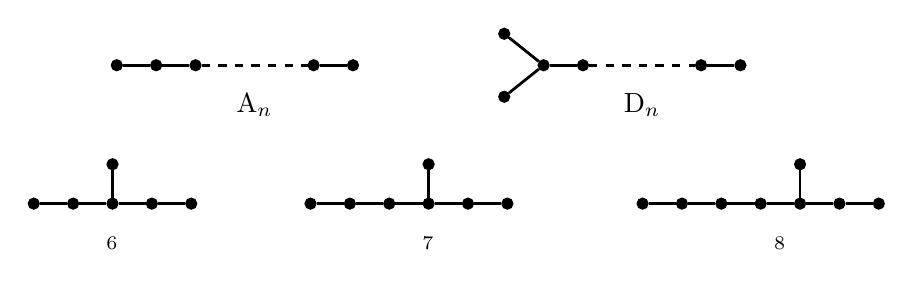
\begin{tikzpicture}
		\tikzset{dynode/.style={circle, draw, fill=black,
					minimum size=4pt, inner sep=0pt}}
		\tikzset{dyline/.style={line width=1pt}}
		\tikzset{dydash/.style={line width=1pt, dashed}}

		\begin{scope}[yshift=0, xshift=22em]
			\node[dynode] (a1) at (0,0) {};
			\node[dynode] (a2) at (0.5,0) {};
			\node[dynode] (a3) at (1,0) {};
			\node[dynode] (a4) at (1.5,0) {};
			\node[dynode] (a5) at (2,0) {};
			\node[dynode] (a6) at (2.5,0) {};
			\node[dynode] (a7) at (3,0) {};
			\node[dynode] (a8) at (2,0.5) {};

			\draw[dyline] (a1) -- (a2) -- (a3) -- (a4) -- (a5) -- (a6) -- (a7);
			\draw[dyline] (a5) -- (a8);

			\node[] (l) at (1.75,-0.5) {$\E_8$};
		\end{scope}

		\begin{scope}[yshift=0, xshift=10em]
			\node[dynode] (a1) at (0,0) {};
			\node[dynode] (a2) at (0.5,0) {};
			\node[dynode] (a3) at (1,0) {};
			\node[dynode] (a4) at (1.5,0) {};
			\node[dynode] (a5) at (2,0) {};
			\node[dynode] (a6) at (2.5,0) {};
			\node[dynode] (a8) at (1.5,0.5) {};

			\draw[dyline] (a1) -- (a2) -- (a3) -- (a4) -- (a5) -- (a6);
			\draw[dyline] (a4) -- (a8);

			\node[] (l) at (1.5,-0.5) {$\E_7$};
		\end{scope}

		\begin{scope}[yshift=0, xshift=0]
			\node[dynode] (a1) at (0,0) {};
			\node[dynode] (a2) at (0.5,0) {};
			\node[dynode] (a3) at (1,0) {};
			\node[dynode] (a4) at (1.5,0) {};
			\node[dynode] (a5) at (2,0) {};
			\node[dynode] (a8) at (1,0.5) {};

			\draw[dyline] (a1) -- (a2) -- (a3) -- (a4) -- (a5);
			\draw[dyline] (a3) -- (a8);

			\node[] (l) at (1,-0.5) {$\E_6$};
		\end{scope}

		\begin{scope}[yshift=5em, xshift=3em]
			\node[dynode] (a1) at (0,0) {};
			\node[dynode] (a3) at (0.5,0) {};
			\node[dynode] (a4) at (1,0) {};
			\node[dynode] (a5) at (2.5,0) {};
			\node[dynode] (a6) at (3.0,0) {};

			\draw[dyline] (a1) -- (a3) -- (a4);
			\draw[dydash] (a4) -- (a5);
			\draw[dyline] (a5) -- (a6);

			\node[] (l) at (1.75,-0.5) {$\mathrm{A}_n$};
		\end{scope}

		\begin{scope}[yshift=5em, xshift=17em]
			\node[dynode] (a1) at (0,0.4) {};
			\node[dynode] (a2) at (0,-0.4) {};
			\node[dynode] (a3) at (0.5,0) {};
			\node[dynode] (a4) at (1,0) {};
			\node[dynode] (a5) at (2.5,0) {};
			\node[dynode] (a6) at (3.0,0) {};

			\draw[dyline] (a1) -- (a3);
			\draw[dyline] (a2) -- (a3);
			\draw[dyline] (a3) -- (a4);
			\draw[dydash] (a4) -- (a5);
			\draw[dyline] (a5) -- (a6);

			\node[] (l) at (1.75,-0.5) {$\mathrm{D}_n$};
		\end{scope}
	\end{tikzpicture}
	\vspace{1em}
	\caption{Dynkin diagrams associated to simple Lie groups.} \label{fig:dynkin-diagram-trees}
\end{figure}

A rich source of trees by which to construct plumbed manifolds are the Dynkin diagrams associated to root systems, see \cref{fig:dynkin-diagram-trees} for the complete set of undirected Dynkin diagrams. There is a deep connection between Dynkin diagrams and the classification of simple Lie groups -- $\mathrm{A}_n$ corresponds to $\SU_{n+1}$, $\mathrm{D}_n$ corresponds to $\SO_{2n}$, and $\E_6, \E_7, \E_8$ correspond to exceptional Lie groups of dimensions 78, 133, and 248 respectively.
A complete discussion of this beautiful topic would take us too far afield, so we refer to Chapter~21 of Fulton and Harris's book \cite{fultonharris1991representation} or to Chapter~3 of Humphrey's book \cite{humphreys1972representation}.

\begin{example}
	If we weight each vertex by $2$, the symmetric bilinear form associated to the $\E_8$ Dynkin diagram has the matrix form
	\[
		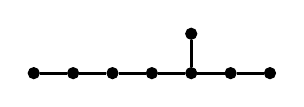
\begin{tikzpicture}
			\tikzset{dynode/.style={circle, draw, fill=black,
						minimum size=4pt, inner sep=0pt}}
			\tikzset{dyline/.style={line width=1pt}}
			\tikzset{dydash/.style={line width=1pt, dashed}}

			\begin{scope}[yshift=-10em, xshift=0]
				\node[dynode] (a1) at (0,0) {};
				\node[dynode] (a2) at (0.5,0) {};
				\node[dynode] (a3) at (1,0) {};
				\node[dynode] (a4) at (1.5,0) {};
				\node[dynode] (a5) at (2,0) {};
				\node[dynode] (a6) at (2.5,0) {};
				\node[dynode] (a7) at (3,0) {};
				\node[dynode] (a8) at (2,0.5) {};

				\draw[dyline] (a1) -- (a2) -- (a3) -- (a4) -- (a5) -- (a6) -- (a7);
				\draw[dyline] (a5) -- (a8);
			\end{scope}
		\end{tikzpicture}
		\quad\lkxto\quad
		\begin{pmatrix}
			2 & 1 &   &   &   &   &   &   \\
			1 & 2 & 1 &   &   &   &   &   \\
			  & 1 & 2 & 1 &   &   &   &   \\
			  &   & 1 & 2 & 1 &   &   &   \\
			  &   &   & 1 & 2 & 1 & 0 & 1 \\
			  &   &   &   & 1 & 2 & 1 & 0 \\
			  &   &   &   & 0 & 1 & 2 & 0 \\
			  &   &   &   & 1 & 0 & 0 & 2 \\
		\end{pmatrix}
	\]
	We will call this the \defn{$E_8$ matrix}.
\end{example}

This matrix is extremely important in differential topology for the following reason:
\begin{proposition}
	The $E_8$ matrix is even, and positive definite, and unimodular.
\end{proposition}
\begin{proof}
	Evenness and positive definiteness are immediate. For the determinant, we could compute it by hand using a series of row/column operations of the form $Q\mapsto PQP^\intercal$ to get
	\[
		\begin{pmatrix}
			2 & 1 &   &   &   &   &   &   \\
			1 & 2 & 1 &   &   &   &   &   \\
			  & 1 & 2 & 1 &   &   &   &   \\
			  &   & 1 & 2 & 1 &   &   &   \\
			  &   &   & 1 & 2 & 1 & 0 & 1 \\
			  &   &   &   & 1 & 2 & 1 & 0 \\
			  &   &   &   & 0 & 1 & 2 & 0 \\
			  &   &   &   & 1 & 0 & 0 & 2 \\
		\end{pmatrix}
		\lkxto
		\begin{pmatrix}
			2 &             &             &             &              &             &             &   \\
			  & \frac{3}{2} &             &             &              &             &             &   \\
			  &             & \frac{4}{3} &             &              &             &             &   \\
			  &             &             & \frac{5}{4} &              &             &             &   \\
			  &             &             &             & \frac{7}{10} &             &             &   \\
			  &             &             &             &              & \frac{4}{7} &             &   \\
			  &             &             &             &              &             & \frac{1}{4} &   \\
			  &             &             &             &              &             &             & 2 \\
		\end{pmatrix}
	\]
\end{proof}

\begin{remark}\label{rmk:E8-manifold}
	The $E_8$ matrix implies that there exists a closed orientable topological $4$-manifold with no smooth structure. \todo{explain} \cite{freedman1982manifold}
\end{remark}

\subsection{Symmetric Bilinear Forms and Lattices}

A common source of symmetric bilinear forms over the integers arise from lattices in an inner product space, such as Euclidean or Lorentzian space. If $(V,\langle -,-\rangle)$ is an inner product space, a lattice $\Lambda\subset V$ inherits the bilinear form $\langle -,-\rangle$. However, this form is generally not integer valued. Some very specially constructed lattices however do inherit an integer valued bilinear form.

For instance, in Euclidean space $\R^\ell$ with basis $\{e_1,\ldots, e_\ell\}$ consider the lattice
\[
	\Gamma^\ell = \span\left\{\frac{1}{2}(e_1+\cdots + e_\ell), e_i+e_j \mid i<j\right\}.
\]
When $4\mid \ell$, the Euclidean inner product restricts to an integral bilinear form on this lattice since
\[
	\begin{aligned}
		\left\langle \frac{1}{2}(e_1+\cdots+e_\ell), \frac{1}{2}(e_1+\cdots+e_\ell)\right\rangle & = \frac{\ell}{4},                                      \\
		\left\langle \frac{1}{2}(e_1+\cdots+e_\ell), e_i+e_j\right\rangle                        & = 1,                                                   \\
		\langle e_i+e_j, e_p +e_q\rangle                                                         & = \delta_{i,p}+\delta_{i,q}+\delta_{j,p}+\delta_{j,q},
	\end{aligned}
\]
where $\delta$ denotes the Kronecker delta. Since the Euclidean inner product is positive-definite, so is the bilinear form of this lattice. When $8\mid\ell$, the bilinear form of this lattice is even, otherwise it is odd. \todo{finish}

A special thing happens when $\ell=8$; in this case the lattice becomes unimodular. 

\begin{theorem}[Mordell]
	The lattice $E_8=\Gamma^8$ is the only even unimodular positive-definite lattice of rank $8$.
\end{theorem}
\begin{proof}
	\todo{cite}
\end{proof}

In fact, $E_8$ is the smallest even unimodular positive-definite lattice.
\begin{theorem}
	The signature of an even unimodular bilinear form is divisible by $8$.
\end{theorem}
\begin{proof}
	\todo{introduce characteristic elements}
\end{proof}

The attractive properties of the $E_8$ lattice make it a great source of inspiration for topological constructions, however we would like to emphasize that it does show up naturally in ``the wild''. For instance:

\begin{example}
	The \defn{Kummer K3 surface} defined by the homogeneous polynomial
	\[
		\textrm{K3} = \left\{ [z_0 : z_1 : z_2 : z_3]\in \CP^3 \mid z_0^4 + z_1^4+z_2^4 + z_3^4=0\right\}
	\]
	has the intersection form $Q_{\textrm{K3}} = E_8\oplus E_8 \oplus^3 H$ of signature 16 and rank 22.
\end{example}

While the classification of definite forms is far more complicated, we already have all of the tools to form a complete list of indefinite forms. First, we can prove that:

\begin{theorem}\label{thm:indefinite-bilinear-forms-isomorphic}
	Two unimodular indefinite bilinear forms are isomorphic if they have the same rank, parity, and signature.
\end{theorem}
\begin{proof}
\end{proof}

We are now equipped to list all of the unimodular indefinite forms.
\begin{proposition}
	Every unimodular indefinite form is isomorphic to either
	\[
		\oplus^p (1)\oplus^q (-1)
		\quad\textrm{or}\quad
		\pm \oplus^r E_8 \oplus^{s>0} H.
	\]
	for some integers $p,q,r,s$. The left side represents all possible odd unimodualr indefinite forms and the right side represents all possible even unimodular indefinite forms.
\end{proposition}
\begin{proof}
	The form $\oplus^p (1)\oplus^q(-1)$ has rank $p+q$ and signature $p-q$, so any rank and signature can be achieved which by \cref{thm:indefinite-bilinear-forms-isomorphic} implies that every odd unimodular \todo{finish}
\end{proof}

\todo{finish}

\subsection{Skew-Symmetric Bilinear Forms}

In the case of skew-symmetric bilinear forms, the structure is far simpler.

\pagebreak
\section{Brieskorn Varieties}\label{sec:brieskorn}
\cite{milnor1968hypersurfaces}
\cite{kauffman1987knots}
